\documentclass{beamer}

\usepackage[ngerman]{babel}
\usepackage[T1]{fontenc}
\usepackage{graphicx}
\usepackage{verbatim}
\usepackage{mdwlist}
\usepackage{listings}
\usepackage{ragged2e}

\usepackage{xunicode}
\usepackage{xltxtra}
\defaultfontfeatures{Mapping=tex-text}
\setmonofont[Mapping={}, Scale=MatchLowercase]{DejaVu Sans Mono}
\setsansfont[Scale=MatchLowercase]{Linux Biolinum O}
\setmainfont[]{Linux Libertine O}

\newbox\mytempbox
\newdimen\mytempdimen
\newcommand\includegraphicscopyright[3][]{%
  \leavevmode\vbox{\vskip3pt\raggedright\setbox\mytempbox=\hbox{%
  \includegraphics[#1]{#2}}%
    \mytempdimen=\wd\mytempbox\box\mytempbox\par\vskip1pt%
    \fontsize{3}{3.5}\selectfont{\color{black!25}{\vbox{\hsize=\mytempdimen#3}}}\vskip3pt%
}}

%\let\raggedright=\RaggedRight
%\hyphenation{Freeze}

\newcommand\prelim[1]{\small }

\newcommand\strColor[1]{\color{beamer@blendedblue}{#1}}

\newcommand\sect[1]{\begin{center}\huge\strColor{#1}\end{center}}

\setbeamerfont{page number in head/foot}{size=\large}
\setbeamertemplate{navigation symbols}{}
\setbeamertemplate{headline}
{%
    \begin{beamercolorbox}{section in head/foot}
        \vskip1em
        \insertsection\hfill
\includegraphics[height=5em]{FULogo_RGB.eps}\hspace{1em}
        \vskip-5.3em
    \end{beamercolorbox}%
}
\setbeamertemplate{footline}[frame number]

\title{OParl-Validator}
\author{Das OParl-Validator-Team}
\institute{Freie Universität Berlin\\Institut für Informatik}
\date{8. Dezember 2014}

\begin{document}

\frame{\titlepage}

%\frame{\tableofcontents}

\frame{
    \frametitle{Gliederung}
    \begin{itemize}
        \item Organisation
        \item Architektur
        \item Features
        \item Close-Out-Plan
        \item Demo
    \end{itemize}
}

\frame{
    \frametitle{Organisation}
    \begin{itemize}[<+->]
        \item Unsere Kunden
        \item Unsere Arbeitsweise: Fazit
        \item Unsere Milestones: Fazit
     \end{itemize}
}

\frame{
    \frametitle{Unsere Kunden}
    \begin{itemize}[<+->]
        \item Direkt
            \begin{itemize}[<*>]
                \item OParl-Entwickler
                \begin{itemize}
                    \item Hauptsächlich Marian (aus Köln, Lucas hat ihn getroffen)
                \end{itemize}
                \item Community
                \begin{itemize}
                    \item Andreas (Semantic-Web-Consultant)
                    \item Stefan
                \end{itemize}
            \end{itemize}
        \item Indirekt
            \begin{itemize}
                \item CC e-Gov GmbH
                \item PROVOX Systemplanung GmbH
                \item QuinScape GmbH
                \item Somacos GmbH und Co. KG
                \item Sternberg Software-Technik GmbH
                \item Zukünftige Projekte, welche den OParl verwenden wollen
            \end{itemize}
    \end{itemize}
}

\frame{
\frametitle{Unsere Arbeitsweise: Fazit}
    \begin{itemize}[<+->]
        \item Kein Vertrag freies miteinander Arbeiten: 
        \begin{itemize}[<*>]
            \item Verantwortlicher sollte bestimmt werden
        \end{itemize}
        \item Regelmäßige Treffen Mittwochs, bei denen auch die Kunden mittels Telefon eingebunden werden:
        \begin{itemize}[<*>]
            \item Zur lückenlosen Zusammenarbeit sehr förderlich
            \item Telefonate haben sich als sehr Zeitaufwändig herausgestellt
            \item Eventuell sollten Telefonate mit dem Kunden nur von einem Projektteilnehemer durchgeführt werden
            \item Alternativ: mehr Mumblen
        \end{itemize}
        \item Eine regelmäßige Telefonkonferenz am Freitag, bei der auch unsere Kunden eingebunden werden
        \begin{itemize}[<*>]
            \item hat sich als sehr hilfreich erwiesen
        \end{itemize}
        \item Kanban
        \begin{itemize}[<*>]
            \item Hat durch die Verwendung von Trello gut funktioniert
            \item Es müssten mehr Boards angelegt werden
            \item Konsequentere Verwendung von Trello
            \item Teilweise schwer geeignete Aufgaben zu finden
        \end{itemize}
        \item Mailingliste
        \begin{itemize}[<*>]
            \item Sehr hilfreiches Mittel
        \end{itemize}   
        \item Hackathons bei Spline:
        \begin{itemize}[<*>]
            \item Sehr produktiv
            \item Generell mehr gemeinsames Coden
        \end{itemize}
        \item Protokollierung der Meetings
        \begin{itemize}[<*>]
            \item Vereinfacht es  Übersicht zu behalten
            \item Hilft bei der Dokumentation 
        \end{itemize}
    \end{itemize}
}

\frame{
    \frametitle{Unsere Milestones: Fazit}
    \begin{itemize}[<+->]
        \item 1. »Zwei Wochen nach Projektstart, wollen wir zwei minimale Projekte in einer Form haben, die es erlaubt sie zu deployen: die Validator-Library wird noch jegliche JSON-Objekte ablehnen, doch ihre Interfaces sollen bereits auf das Frontend-Projekt abgestimmt sein. Das Frontend-Projekt soll eine minimale Eingabemaske für JSON-Objekte zur Verfügung stellen und zur Validierung auf die Library zurückgreifen. Auf diese Seite können wir den Product Owners bereits Zugriff gewähren.«
        \begin{itemize}[<*>]
             \item Frontend auf Wunsch der Kunden zurückgestellt
             \item JSON-Objekte konnten, wei geplant, über das CLI eingegeben und von der Library getestet werden
        \end{itemize}
        \item 2. »Ein existierender Server, der Testdaten ausliefert, soll erweitert worden sein, und der Validator soll bereits grundlegende Tests durchführen können. Das Web-Frontend soll derweil benutzerfreundlicher sein, ins besondere im Bezug auf die Fehlerberichterstattung.«
        \begin{itemize}[<*>]
            \item Es wurden grundlegende Server Tests implementiert
        \end{itemize}
        \item 3. »Gerade alle syntaktisch korrekten Objekte sollen akzeptiert werden, und das Frontend-Projekt soll auch JSONs über HTTP und HTTPS abrufen und validieren können.«
        \begin{itemize}[<*>]
            \item Diskussion über die Unterstützung von JSON-LD verlansamte unsere Arbeit
            \item Objekte können mit einer URL eingebunden und validiert werden
        \end{itemize}   
        \item 4. »Der Validator soll auch JSON-LD-Referenzen validieren, auch unter Beachtung von Weltwissen über die in den JSON-Objekten abgebildeten politischen Körper. Das Frontend-Projekt soll Hilfestellungen zur Lösung typischer Fehler leisten.«
        \begin{itemize}[<*>]
            \item JSON-LD wird nicht komplett unterstützt
            \item es wurden spezielle Tests für die Fälle Entwickelt, die JSON-Schema nicht prüfen kann
        \end{itemize}   
        \item 5. »Um Hierarchien von Objekten vollständig und stichpunktartig validieren zu können, soll ein Crawler eine größere Anzahl von JSON-Objekten gezielt abrufen und in Bezugnahme aufeinander validieren können.«
        \begin{itemize}[<*>]
             \item Der Crawler kann LD-Struktur durchsuchen und die Objekte validieren
        \end{itemize}   
    \end{itemize}
}

\frame{
    \frametitle{Features}
    \begin{itemize}[<+->]
        \item Continuous Integration
        \begin{itemize}[<*>]
            \item Dank Travis CI
            \item Mit automatischer Coverage dank Coveralls
        \end{itemize}
        \item Python 2.7 und 3.3+
        \begin{itemize}[<*>]
            \item \texttt{six}-Library sehr hilfreich
            \item Continuous Integration ebenso
        \end{itemize}
        \item Constraints
        \begin{itemize}[<*>]
            \item Type Whitelist, Rekursion, etc.
        \end{itemize}
    \end{itemize}
}

\frame{
    \frametitle{Featureprobleme und -lösungen}
    \begin{itemize}[<+->]
        \item Python 2.7 vs. Python 3.3+ vs. beide
        \begin{itemize}[<*>]
            \item Python 2.7: Noch weiter verbreitet, wird nicht mehr weiterentwickelt
            \item Python 3.3+: Die Zukunft, besser, wird weiterentwickelt
            \item \textbf{Beide}: Verschieden umsetzbar, komplexer
        \end{itemize}
        \item QA mit beiden Versionen umständlich
        \begin{itemize}[<*>]
            \item Travis CI führt die Tests mit beiden Versionen nach jedem Push aus
        \end{itemize}
    \end{itemize}
}

\frame{
    \frametitle{Demo}
    Slide mit Absicht leer – mit Ausnahme der Überschrift, des FU-Logos, des Foliums und dieses Textes
}

\frame{
    \frametitle{Architektur}
    \begin{columns}
        \begin{column}{.6\textwidth}
            \begin{itemize}[<+->]
                \item Command Line Interface
                \begin{itemize}[<*>]
                    \item Gemeinsamer Entry-Point
                \end{itemize}
                \item Crawler
                \begin{itemize}[<*>]
                    \item Validiert ein komplettes System
                    \item Oder einen Teil des Systems
                \end{itemize}
                \item Server-Tests
                \begin{itemize}[<*>]
                    \item Suite mit Anforderungen auf tieferer Abstraktionsebene
                    \item Aber auf Layer 7
                \end{itemize}
                \item Validator
                \begin{itemize}[<*>]
                    \item Basierend auf Freeze vom 22. Juli
                    \item Mit einigen optionalen Features
                \end{itemize}
            \end{itemize}
        \end{column}
        \begin{column}{.4\textwidth}
            \hspace{-1cm}
            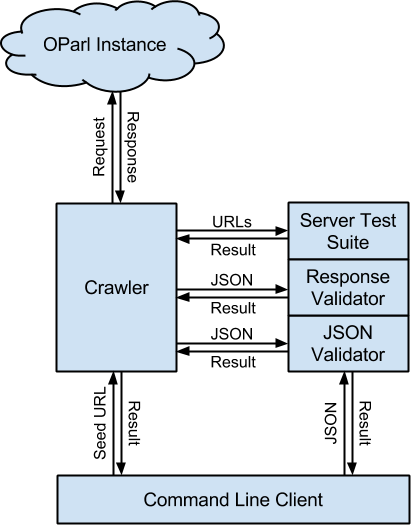
\includegraphics[width=1.2\textwidth]{architecture.final.png}
        \end{column}
    \end{columns}
}

\frame{
    \frametitle{Architekturprobleme und -lösungen}
    \begin{itemize}[<+->]
        \item JSON- vs. Dict-Validierung
        \begin{itemize}[<*>]
            \item Dict: Vereinfacht den Code im Validator
            \item \textbf{JSON}: Erlaubt zentrale Behandlung von Fehlern im Validator
        \end{itemize}
        \item Server-Tests
        \begin{itemize}[<*>]
            \item Parallel: Beste Abdeckung aber unzählige Requests
            \item \textbf{Final}: Schneller, flexibler, aber erfordert Sammlung der URLs
        \end{itemize}
        \item Paralleles oder finales Reporting
        \begin{itemize}[<*>]
            \item \textbf{Parallel}: Der Benutzer kann abbrechen und bereits gefundene Fehler beheben
            \begin{itemize}[<*>]
                \item Einfach durch Generatoren in Python umsetzbar
            \end{itemize}
            \item Final: Spart ein paar Zeilen Code
        \end{itemize}
    \end{itemize}
}

\frame{
    \frametitle{Close-Out-Plan}
    \begin{itemize}[<+->]
        \item OParl 1.0 noch nicht finalisiert
        \item Einige des Teams werden die letzten Anpassungen zu gegebener Zeit vornehmen
        \item Einige des Teams werden das Projekt auch langfristig zusammen warten
    \end{itemize}
}

\end{document}
